\subsection{Following the commands rather than the proxy}
The next step is to ask what the controller actually does. The pinned simulator provides observers that count each issued command and, for the microbenchmark, record its cycle and decoded address. Replaying with these observers gives exactly the same cycles and row-hit counts as the original runs. The observers add evidence without changing the simulated schedule.

Table~\ref{tab:microcommands} gives an exact accounting for this controller. Because it selects at most one command per cycle,
\begin{equation}
 T = N_{\text{command cycles}} + N_{\text{no-command cycles}}.
\end{equation}
A command cycle may open or close a row, issue a read, or perform refresh. A no-command cycle can arise from timing restrictions, a lack of eligible work, or draining the last reads. It is deliberately not labelled as a particular stall cause.

\begin{table}[htbp]\centering\small
\caption[Command accounting for request order]{Controlled ordering experiment with command observers. ACT opens a row; PRE combines per-bank and all-bank precharge commands. The read count is 16,384 in every row. ``Limit'' is the maximum number of outstanding reads.}\label{tab:microcommands}
\begin{tabular}{rlrrrr}
\toprule
Limit & Order & Cycles & ACT & PRE & No command \\
\midrule
64 & Sequential & 30894 & 528 & 38 & 13930 \\
64 & Permuted & 28968 & 3793 & 3319 & 5458 \\
1 & Sequential & 325786 & 588 & 166 & 308482 \\
1 & Permuted & 398592 & 4044 & 1135 & 376825 \\
\bottomrule
\end{tabular}

\end{table}

At limit 64, the permutation opens and closes more rows, yet has fewer no-command cycles. The reduction in those cycles exceeds the cost of the extra command-issue cycles. At limit one, no other read can hide the waiting for the current read, and the additional row changes make permutation slower. The two interventions expose the trade-off: reducing commands and overlapping service are different ways to reduce time.

The offered sequential stream spans an average of \SequentialBanks{} different bank instances per sliding window of 64 requests, compared with \RandomBanks{} for the permutation. Each statistic counts complete windows within queries under the verified default mapper. This measures diversity in the input stream; it is not a measurement of how many banks are ready simultaneously, or how many requests occupy the controller queue.

\begin{figure}[htbp]\centering
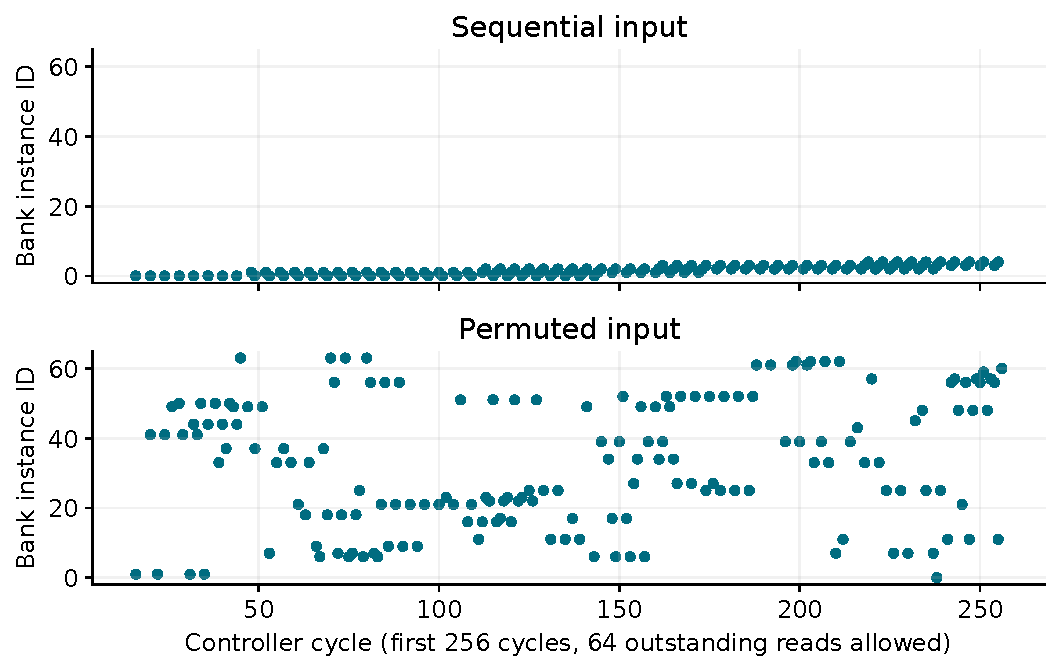
\includegraphics[width=\textwidth]{generated/command_timeline.pdf}
\caption[Read-command timing and bank exposure]{Actual read-command issues in the first 256 controller cycles, with limit 64. Each dot is one RD command; the vertical position identifies its bank instance. Sequential requests concentrate early service in a few banks, while the permutation exposes a wider set. The full-run counts, rather than this short initial interval alone, support the timing comparison.}\label{fig:commands}
\end{figure}

This evidence supports a locality--parallelism explanation for the controlled reversal. It does not assign every saved cycle to an individual timing rule: refresh, buffering and scheduling interact. The important result is that an observed reduction in row operations can be outweighed by the service opportunities lost elsewhere in the schedule.
